\documentclass[12pt]{extarticle}
\usepackage{tikz}
\usepackage{amsmath,amssymb}
\usepackage {graphicx}
\usepackage{multicol}
\usepackage{hyperref}
\usepackage{geometry}
\usepackage{watermark}
\usepackage{varwidth}
\usepackage{arydshln}
\usepackage[dvipsnames]{xcolor}
\usepackage{tcolorbox}
%\usepackage{scrlayer-scrpage}
\usepackage{forest}
\usepackage{fancyhdr}
\pagecolor{white}
 \geometry{bottom= 30mm}
\usepackage{enumitem}


 
 
\title{Data Management Assignment 6}
\author{Janis Waser} 
\fancyhead[L]{Data Management}
\fancyhead[C]{Homework 6}
\fancyhead[R]{ Janis Waser}
\renewcommand\headrulewidth{0pt}
\pagestyle{fancy}
\pagenumbering{arabic}

\begin{document}

\maketitle \vspace{-10mm}
\rule{\linewidth}{0.4pt}


\begin{flushleft}
\begin{enumerate}[label=\textbf{\Alph*.}]

\item 
\begin{enumerate}[label=\arabic*.]
\item \begin{enumerate}[label=(\alph*)]
\item Transaction 4 (T4) needs to be redone, it committed after the last checkpoint and therefore this transaction must be reflected in the final state.
\item Transactions 3,5 and 6 have to be undone. Transaction 3 started before the checkpoint but did not commit before the failure, it has to be undone. As well as transactions T5 and T6 who started after but did not commit and therefore need to be undone. T6 has not yet made an operation as in our system the log is ahead of any operation, so theoretically you can ignore 6 as no operation can be undone.
\item T1 and T2 have committed before the last checkpoint, thus they are not affected by the crash.
\end{enumerate}
 \item \begin{enumerate}[label=(\alph*)] 
\item The possible values of a are 1 or 2, before the last checkpoint it was changed to 1 and after it it was again changed to 2. 

The possible values for b are 2 or 3. The checkpoint insures that after it the disk contains 2 and then b is altered to 3, which we do not know if it actually gets written to the disk. 

Finally, c can be 0 or 1 as it is changed only after the checkpoint and again we cannot know whether the value 1 was written on the disk before the crash. 
\item T1 is ignored, T2 needs to be redone and transaction 3 and 4 undone. Therefore the values of a, b, c are: a=2, b=2, c=0. 
\end{enumerate}
\end{enumerate}
\item 
\begin{enumerate}[label=\arabic*.]
\item \begin{enumerate}[label=(\alph*)]
\item A database history is recoverable if every transaction commits only after all transactions from whom values are read, are already committed. More precisely, the commit of a transaction has to be after all commits of the transaction from whom values are read during this transaction. 
\item A database history is cascadeless if every transaction only reads values from other transactions who have already committed. If a transaction reads a value who was written by a transaction that has not committed then it is not cascadeless.
\item The schedule is strict if a transaction only changes(writes) values who have already committed in all transaction who write to this value and also satiesfies the condition for avoiding cascading aborts(no read from values whose transaction has not committed yet)
\end{enumerate}
\item \begin{enumerate}[label=(\alph*)]
\item It is recoverable as long as T2 commits before T4. y is only written once and this is after being read. z is only read and written by T5 after T3 has committed. 

It is not cascadeless as T2 writes x and without commit of T2, x is read by T4. 

As this schedule already violates the constraint for cascading aborts, it cannot be strict, but the rest would actually be strict as x, y, z are only written once.
\item This history is not recoverable as T1 writes to b, never commits and T4 reads x and writes and commits. 

This history is not cascadeless for the same reason as above but it does not matter whether T4 commits before T1 or not. 

This history cannot be strict as it is not cascadeless and T1 writes to x after T2 wrote to x without committing/aborting.
\end{enumerate}
\end{enumerate}
\item \begin{enumerate}[label=(\alph*)]
\item We draw the conclict graph instruction by instruction and simplify by only considering the transactions: 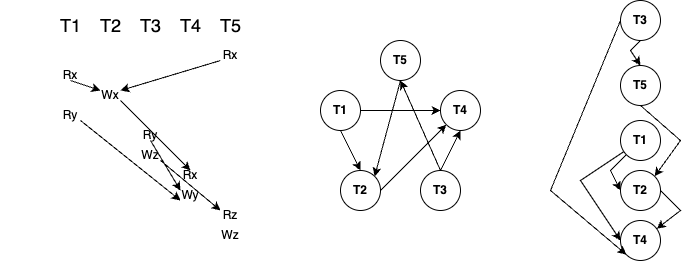
\includegraphics[width=\linewidth]{graph_a}
We see that the graph is acyclic. There are 3 possible sequences: We can start with either T1 or T3. If we start with T3, we can again choose between T1 and T5. If we start with T1 then the order is predetermined. This gives us the following possible serial schedules: $[T1, T3, T5, T2, T4 ] \quad or\quad [T3, T1, T5, T2, T4 ] \quad or \quad  [T3,  T5, T1,T2, T4 ] $
We can see that all this orders work:
 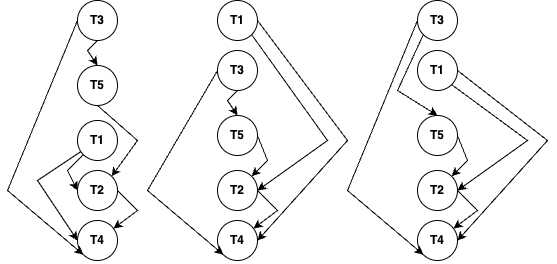
\includegraphics[width=\linewidth]{serial_example_a}
\item We repeat the same process to get the serialisablility graph:
 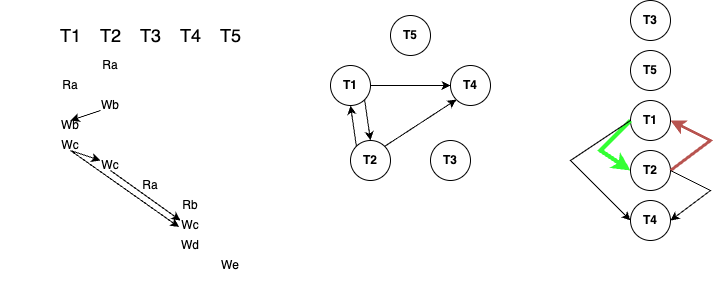
\includegraphics[width=\linewidth]{graph_b}
 We see that there exists a circle from T1 to T2. In whatever order we put T1 and T2, we will create a problem e.g. the example $[T3,  T5, T1,T2, T4 ] $ has a conflict (shown in red).
\end{enumerate}

\end{enumerate}
\end{flushleft}
\end {document}